\documentclass{article}

\usepackage{amsmath,amssymb,amsthm,latexsym,color} %Basic packages
\usepackage{dsfont} % bb fonts for numbers
\usepackage{braket} % nice sets and more
\usepackage{accents}
\usepackage{musicography}
\usepackage{biblatex} % TODO: [citestyle=mla] causes compilation error
\usepackage{graphicx}
\usepackage[nice]{nicefrac}
\allowdisplaybreaks[2] %Allow page breaks in multi-line displays
\usepackage{xspace} % smart whitespacing after commands
\usepackage{mathtools}

%%%%%%%%%%%%%%%%%%%%%%%%%%%%%%%%%%%%%%%%%%%%%%%%%%%%%%%%%%%%%%%%%%%%%%
%Swaps the roles of phi and epsilon with the var versions
\let\temp\phi
\let\phi\varphi
\let\varphi\temp

\let\temp\epsilon
\let\epsilon\varepsilon
\let\varepsilon\temp
%%%%%%%%%%%%%%%%%%%%%%%%%%%%%%%%%%%%%%%%%%%%%%%%%%%%%%%%%%%%%%%%%%%%%%


%%%%%%%%%%%%%%%%%%%%%%%%%%%%%%%%%%%%%%%%%%%%%%%%%%%%%%%%%%%%%%%%%%%%%%
%Shorthand 
\newcommand{\seq}[1]{\{#1\}}
\newcommand{\linf}{\lim_{n \to \infty}}
\newcommand{\Alpha}{\mathcal{A}}
\newcommand{\ubar}[1]{\underaccent{\bar}{#1}}
\newcommand{\norm}[1]{\left\lVert#1\right\rVert}

\newcommand{\limnf}[1]{\liminf \limits_{#1}}
\newcommand{\limsp}[1]{\limsup \limits_{#1}}
\newcommand{\lone}{L^1}

\newcommand{\kph}{\ensuremath{\ket{\phi}}\xspace}
\newcommand{\kphind}{\ensuremath{\ket{\phi_i}}\xspace}
\newcommand{\kpho}{\ensuremath{\ket{\phi_0}}\xspace}
\newcommand{\kphi}{\ensuremath{\ket{\phi_1}}\xspace}
\newcommand{\kphii}{\ensuremath{\ket{\phi_2}}\xspace}
\newcommand{\ko}{\ensuremath{\ket{0}}\xspace}
\newcommand{\ki}{\ensuremath{\ket{1}}\xspace}
\newcommand{\koo}{\ensuremath{\ket{00}}\xspace}
\newcommand{\kio}{\ensuremath{\ket{10}}\xspace}
\newcommand{\koi}{\ensuremath{\ket{01}}\xspace}
\newcommand{\kii}{\ensuremath{\ket{11}}\xspace}

\newcommand{\Mod}[1]{\ (\mathrm{mod}\ #1)}

%%%%%%%%%%%%%%%%%%%%%%%%%%%%%%%%%%%%%%%%%%%%%%%%%%%%%%%%%%%%%%%%%%%%%%

%%%%%%%%%%%%%%%%%%%%%%%%%%%%%%%%%%%%%%%%%%%%%%%%%%%%%%%%%%%%%%%%%%%%%%
%Shorhands for commond blackboard bold symbols
\newcommand{\R}{\ensuremath{\mathbb R}}
\newcommand{\C}{\ensuremath{\mathbb C}}
\newcommand{\N}{\ensuremath{\mathbb N}}
\newcommand{\Q}{\ensuremath{\mathbb Q}}
\newcommand{\Z}{\ensuremath{\mathbb Z}}
%%%%%%%%%%%%%%%%%%%%%%%%%%%%%%%%%%%%%%%%%%%%%%%%%%%%%%%%%%%%%%%%%%%%%%

%%%%%%%%%%%%%%%%%%%%%%%%%%%%%%%%%%%%%%%%%%%%%%%%%%%%%%%%%%%%%%%%%%%%%%
%Used to alerting the reader
\newcommand{\nb}[1]{{\color{red}{$\clubsuit$#1$\clubsuit$}}}
%%%%%%%%%%%%%%%%%%%%%%%%%%%%%%%%%%%%%%%%%%%%%%%%%%%%%%%%%%%%%%%%%%%%%%

%%%%%%%%%%%%%%%%%%%%%%%%%%%%%%%%%%%%%%%%%%%%%%%%%%%%%%%%%%%%%%%%%%%%%%
%Theorem environments
\theoremstyle{definition}
\newtheorem{soln}{Solution}
\newtheorem{defn}{Definition}[soln]
\newtheorem{post}{Postulate}
\numberwithin{defn}{section}

\theoremstyle{plain}
\newtheorem{theo}{Theorem}[soln]
\newtheorem{prop}{Proposition}[soln]
\newtheorem{lem}{Lemma}[soln]
\newtheorem{claim}{Claim}[soln]
\newtheorem{cor}{Corollary}[soln]
\newtheorem*{exercise*}{Exercise}


\theoremstyle{remark}
\newtheorem{rem}{Remark}[soln]
\numberwithin{rem}{section}
%%%%%%%%%%%%%%%%%%%%%%%%%%%%%%%%%%%%%%%%%%%%%%%%%%%%%%%%%%%%%%%%%%%%%%



%%%%%%%%%%%%%%%%%%%%%%%%%%%%%%%%%%%%%%%%%%%%%%%%%%%%%%%%%%%%%%%%%%%%%%
\bibliography{citations}
%%%%%%%%%%%%%%%%%%%%%%%%%%%%%%%%%%%%%%%%%%%%%%%%%%%%%%%%%%%%%%%%%%%%%%

\begin{document}
\title{Quantum Computation -- CS 7805 Lecture Notes}

\author{Artem Pelenitsyn and Max Daniels}

\date{\today}

\maketitle

\tableofcontents 

\section*{Introduction}

The works of Paul Benioff, Richard Feynman, and Yuri Manin
from early 1980-s presented the idea of using the effects of quantum
mechanics in computation. By 1994, Peter Shor came up with an idea
and design of a quantum polynomial-time algorithm for factoring integer
numbers~--- the problem without an efficient (probabilistic or
deterministic) solution to this date.

The essence of the speedup achieved lies in so called \emph{quantum parallelism}~---
an observation that the computational space increases exponentially with
the size of the quantum system. One more (quantum) bit of input allows for computation
over two times more of states simultaneously.

Quantum parallelism
does not come for free, though: at the end of computation you have to ``measure''
its result; this will collapse all parallel states into a single one with a certain 
probability. Only certain algorithm designs can benefit from this style 
of parallel probabilistic computation.


\section{Computational Model}

\subsection{Quantum Information: Qbits}

We define the representation of information we are going to compute over as follows.

\begin{post}[State Space Postulate]
The state of a system is described by a unit vector in a Hilbert space $\mathcal H$.
\end{post}

The word ``system'' here refers to some physical reality used to encode information,
akin to transistors used to encode classical bits. A quantum system can be implemented
with some elementary particle and its property. E.g. an electron and its spin, a photon
and its polarization, etc.

Recall that a Hilbert space is a complex linear space with a scalar product structure
on it. Hilbert space can have infinite dimensions and that is often the case when
working out quantum mechanics but for the purpose of quantum computing it suffices to
employ the finite-dimensional case.

For a finite-dimensinal $\mathcal H$: there is a natural number $n$ such that 
$\dim(\mathcal H) =n$. The dimensionality depends on the degree of freedom of 
the concrete system. We will assume that we have
at our disposal an unbounded number of replicas of a 2-dimensional system, which 
(for the reasons explained later) we will call \textit{qubits}.

A state of a qubit, therefore, is described by a pair of complex numbers (a member 
of the coordinate space $\C^2$) and a choice of
basis in the state space. We assume that there exists the standard basis which we denote
$\ket 0$, $\ket 1$. E.g. if our concrete realization of qubits is the spin characteristic
of an electron, the usual choice of the basis would be: $\ket 0$ for spin-up
and $\ket 1$ for spin-down. 

The algebraic form describing a state of a qubit is:
\[
  \alpha_0 \ket 0 + \alpha_1 \ket 1, \qquad \alpha_i \in \C: |\alpha_0|^2 + |\alpha_1|^2 = 1.
\]
We usually call $\alpha_i$ the \textit{amplitudes}. They are complex numbers although
there is a theoretical result stating that we can limit ourselves to real numbers without
a loss of generality. In that case, the state of a qubit can be pictured as a
point on the unit circle.

\paragraph{Takeaway} Our elementary piece of information, qubit, is a unit vector
in a complex two-dimensional space.

\subsection{Quantum Computation: Unitary Transformations}

Given that qubits live in a sort of linear space, one would expect possible
manipulations with them to preserve the linear structure. This is, indeed, 
the case.

One essential constraint attached to qubits is the unit length of the 
corresponding vectors. Therefore, the said transformations should
preserve lengths.

Combining the two ideas we get to the Evolution Postulate.


\begin{post}[Evolution Postulate]
The time-evolution of the state of a closed quantum system is described
by a \emph{unitary operator}.
\end{post}

In the finite-dimensional case (which is of main interest for us) unitary
operators simply correspond to isometries (a linear transformation 
preserving lengths). In general, the definition is somewhat more involved 
but proves to be useful in showing even finite-dimensional operators unitary.

Unitary operators are those that preserve not only lengths but also angles.
Recall that angles are measured with scalar product, so
\[
  U \text{— unitary} \Leftrightarrow (Ux,Uy) = (x,y).
\]
Recalling that one can shuffle around the action of an operator around the
scalar product using the notion of adjoint operator, 
\[
  (Ux,Uy) = (x,U^*Uy),
\]
we can get an to an equivalent formulation:
\[
  U \text{— unitary} \Leftrightarrow U^*=U^{-1}.
\]

This formulation is sometimes easier to check in a finite-dimensional 
case. Recall that in terms of matrices $U^* = \seq{U_{ji}^*}$, 
where $U_{ij}$ is $i,j$-th element of $U$ and $a^*$ is the complex 
conjugate of $a$. Therefore, for real matrices (which we will mostly deal with),
we want the matrix of the inverse operator to be equal to the trasposition of
the matrix of the operator itself. Moreover, if a real operator is an involution
($U^2=I$, i.e. it is self-inverse), then for it to be unitary it suffices to
check that its own matrix is symmetric.

The postulate means that if the state $\ket{\phi_0}$ of a qubit evolved over 
time into the state $\ket{\phi_1}$ then there exists a unitary operator $U$, such
that
\[
  \ket{\phi_1} = U \ket{\phi_0}.
\]
All our computations will have to take form of unitary transformations.

One interesting aspect of quantum computing is that it is reversible: given 
the outputs of a quantum circuit we can always rebuild the inputs. This 
should seem very restrictive and indeed it is. But we will see that with
some redundancy in the inputs we can model any classical computation.

\paragraph{Takeaway} We work with qubits by means of isometric linear 
transformations.

\subsection{Composite Systems}

The next postulate provides a way to stack up qbits, similarly to how 
we compose bits into bit-strings (e.g. bytes, registers, etc.) in the 
classical setting.

\begin{post}[Composition of Systems Postulate]
If one system is in the state \kphi and the second system in the state 
\kphii, then the state of the combined system is described by the 
\emph{tensor product}:
\[
    \kphi \otimes \kphii \in \mathcal H_1 \otimes \mathcal H_2,\qquad \text{if }
    \ket{\phi_i}\in\mathcal H_i.
\]
\end{post}

\textbf{Notation} We often omit ${\otimes}$ and write \kphi\kphii or even $\ket{\phi_1\phi_2}$ instead of $\kphi \otimes \kphii$.

It is handy to think about the tensor product as a simple pairing operation which
has only one non-trivial property --- \emph{bilinearity} (that is, it is linear 
in both arguments). So we can hoist and push 
down scalar multipliers and summations through this paring operation.
The following example demonstrates how this works.

Consider two qubits described by
\[
  \kphi = \nicefrac 1 {\sqrt 2} (\ko + \ki), \qquad 
  \kphii = \nicefrac 1 {\sqrt 2} (\ko - \ki).
\]
Considered as a composite system, their collective state is described as follows:
\[
  \kphi \kphii = \nicefrac 1 2 (\ko + \ki) (\ko - \ki) 
    = \nicefrac 1 2 (\ket{00} - \ket{01} +\ket{10} +\ket{11}).
\]
It should be intuitively clear that the resulting composite state of two qubits 
is described with a 4-dimensional vector. In general, $n$-qubit system corresponds
to a vector with $2^n$ dimensions. This is the source of quantum parallelism 
mentioned in the Introduction.

\subsubsection{Entangled States}

A pair of qubit is a system that is described by a 4-dimensional vector.
An intriguing observation first made in this context by Einstein, Podolsky,
and Rosen is that not every such vector can be represented as a product of 
two-dimensional ones. E.g.
\[
  \kph = \nicefrac 1 {\sqrt 2} ( \koo + \kii )
\]
Such a state is indeed achievable from a basis like \koo using a simple unitary
transformation so it should correspond to some valid state of a pair of qubits.
But what are individual states of those qubits? This is not known. Such qubits
are called \emph{entangled} (or \emph{EPR pairs}). The set of entangled qubits 
is dense in the 4-dimensional Hilbert space, so entanglement is not rare: 
``most'' pairs of qubits are entangled. 

We will see that entanglement is among the most important workhorses of quantum
computing.

\paragraph{Takeaway} We stack qubits up by tensoring (qlueing up) the corresponding
state vectors. Not all vectors describing a pair (n-tuple) of qubits are possible
to ``unglue''.

\subsection{Measurement}

We now sched some light on the notion of closed system mentioned in the
previous section and when it comes to odds with our ability to access
the parameters of the system, e.g. the amplitudes.

An important limitation of the model described so far is that the 
amplitudes cannot be recovered by a classical observer (e. g. a human) 
directly. From the classical point of view the possible states of the 
qubit are still either \ko or \ki. Recall the infamous thought 
experiment with the Schr{\"o}dinger's cat: the cat can only be either 
dead or alive but not $\nicefrac 1 {\sqrt 2} \text{ dead} + \nicefrac 1 
{\sqrt 2} \text{ alive}$. Yet this is the kind of states, called 
\emph{superpositions}, quantum mechanics deals with. And a 
superposition can be maintained (and even transformed using the 
Evolution Postualte) as long as the system remains unobserved. Once 
this condition is broken, the system shuts down back to one of 
classical states.

The only way to experience amplitudes requires the act of measurement
that inevitably changes the state of the system.

\begin{post}[Measurement Postulate]
Assume a quantum system $A$ and its corresponding state space $\mathcal H_A$.
For an orthonormal basis $B = \seq{\kphind}$ in $\mathcal H_A$, there exists
a description of $A$:
\[
    \kph = \sum_i \alpha_i\kphind, \qquad \sum_i |\alpha_i|^2 = 1.
\]
It is possible to perform a \emph{(Von Neumann) measurement} on 
system $A$ with respect to the basis $B$. With probability $|\alpha_i|^2$, 
this act outputs a label $i$ and leaves the system in state \kphind.
\end{post}

Consider
a pair of qubits in the state
\[
  \kph 
  = \sqrt{\nicefrac 1 {11}} \koo 
  + \sqrt{\nicefrac 5 {11}} \koi
  + \sqrt{\nicefrac 2 {11}} \kio
  + \sqrt{\nicefrac 3 {11}} \kii .
\]
We can measure the system as a whole using the standard (0/1) basis 
and get $00$ as the output with probability \nicefrac 1 {11}, 
get $01$ with probability \nicefrac 5 {11}, etc. And if we get, say, 01
as the output, then the system ends up in the state \koi.

A measurement can be performed on individual qubits of a system.
Assume we want to measure the first qubit of the above mentioned system using 
the standard basis. From above, we know that the probability of getting
0 for the first qubit is $\nicefrac 1 {11} + \nicefrac 5 {11} = \nicefrac 6 {11}$.
In order to figure out what happens with the whole system after this
measurement with the outcome of 0, we regroup the terms using bilinearity:
\[
  \kph 
  = \sqrt{\nicefrac 6 {11}} \ko \left ( 
    \sqrt{\nicefrac 1 6} \ko + \sqrt{\nicefrac 5 6} \ki
  \right ) +
  \sqrt{\nicefrac 5 {11}} \ki \left ( 
    \sqrt{\nicefrac 2 5} \ko + \sqrt{\nicefrac 3 5} \ki
  \right ).
\]
It is clear that if we get the output 0, the system ends up in the state
\[
  \ko \left ( 
    \sqrt{\nicefrac 1 6} \ko + \sqrt{\nicefrac 5 6} \ki
  \right ).
\]

\section{Quantum Gates}
An $n$-qubit system has $2^n$ basis states. If we map these states to Euclidean basis vectors, the state space is like the points on the unit sphere in $\C^{2^n}$. To interact with these states, we apply \textit{unitary transformations}, which are invertible maps $S^{2^n-1} \mapsto S^{2n-1}$ (geometrically, we need unitarity because we can only map the sphere to itself by twisting it around). 
\subsection{Basic Gates}
Here are some unitary state transformations that act like logic gates. Again, we are implicitly mapping $\ket{0} \to e_0$ and $\ket{1} \to e_1$.
\begin{enumerate}
    \item Identity ($I$ gate):
    \begin{align}
        I = 
        \begin{pmatrix}
            1 & 0 \\
            0 & 1
        \end{pmatrix}
        \ \ \ \
        &
        \begin{cases}
            \ket{0} \to \ket{0} \\
            \ket{1} \to \ket{1}
        \end{cases}
    \end{align}
    \item Swap ($X$ gate):
    \begin{align}
        X = 
        \begin{pmatrix}
            0 & 1 \\
            1 & 0
        \end{pmatrix}
        \ \ \ \
        &
        \begin{cases}
            \ket{0} \to \ket{1} \\
            \ket{1} \to \ket{0}
        \end{cases}
    \end{align}
    \item Swap \& shift ($Y$ gate, $Y=ZX$):
    \begin{align}
        Y = 
        \begin{pmatrix}
            0 & 1 \\
            -1 & 0
        \end{pmatrix}
        \ \ \ \
        &
        \begin{cases}
            \ket{0} \to -\ket{1} \\
            \ket{1} \to \ket{0}
        \end{cases}
    \end{align}
    \item Phase shift ($Z$ gate):
    \begin{align}
        Z = 
        \begin{pmatrix}
            1 & 0 \\
            0 & -1
        \end{pmatrix}
        \ \ \ \
        &
        \begin{cases}
            \ket{0} \to \ket{0} \\
            \ket{1} \to -\ket{1}
        \end{cases}
    \end{align}
    \item Controlled Not ($C_{not}$ gate):
    \begin{align}
        C_{not} = 
        \begin{pmatrix}
            1 & 1 & 0 & 0 \\
            0 & 1 & 0 & 0 \\
            0 & 0 & 0 & 1 \\
            0 & 1 & 1 & 0
        \end{pmatrix}
        \ \ \ \
        &
        \begin{cases}
            \ket{00} \to \ket{00} \\
            \ket{01} \to \ket{01} \\
            \ket{10} \to \ket{11} \\
            \ket{11} \to \ket{10} 
        \end{cases}
    \end{align}
    
    \item Walsh-Hadamard ($H$ gate):
    \begin{align}
        H = 
        \begin{pmatrix}
            \nicefrac{1}{\sqrt{2}} & \nicefrac{1}{\sqrt{2}} \\
            \nicefrac{1}{\sqrt{2}} & -\nicefrac{1}{\sqrt{2}}
        \end{pmatrix}
        \ \ \ \
        &
        \begin{cases}
            \ket{0} \to (\nicefrac{1}{\sqrt{2}})(\ket{0} + \ket{1}) \\
            \ket{1} \to (\nicefrac{1}{\sqrt{2}})(\ket{0} - \ket{1}) \\
        \end{cases}
    \end{align}
    $H$ is a rotation by $\nicefrac{\pi}{4}$ and it superimposes $\ket{0}$ equally over the two states. Applying $H$ iteratively to each bit of $\ket{0^n}$ superimposes equally over all of $\ket{x}, x \in \Set{0, 1}^n$ 
    \begin{prop}
    \begin{equation}
    H_n \ket{x} = \frac{1}{(\sqrt{2})^n} \sum_{y=0}^{2^n - 1} (-1)^{x \odot y} \ket{y}
    \end{equation}
    \end{prop}
    \begin{proof}
    Idea is: For the $n$th bit of $y$, if this bit is zero then its coefficient is $\nicefrac{1}{\sqrt{2}}$. If this bit is one, then its coefficient is $\nicefrac{-1}{\sqrt{n}}$ iff the corresponding $n$th bit of $x$ is $\ket{1}$. The states accumulate a $-1$ factor for every Hadamard-child $\ket{1}$ of a parent $\ket{1}$. The $x\odot y$ counts occurrences of this. Simple example:
    \begin{equation}
        H \ket{01} = \frac{1}{\sqrt{2}} ( \ket{0} + \ket{1} )  \cdot \frac{1}{\sqrt{2}} ( \ket{0} - \ket{1} ) 
    \end{equation}
    \end{proof}
    
\end{enumerate}

\subsection{No Cloning}
\begin{theo}[No Cloning]
There is no unitary $U$ satisfying
\begin{equation}
    U \ket{a0} = \ket{aa} \text{ for all qunatum states $\ket{a}$}
\end{equation}
In this sense, no unitary transformation can clone qubits.
\end{theo}
\begin{proof}
Set $\ket{c} = (\nicefrac{1}{\sqrt{2}})(\ket{a} + \ket{b})$. \\
Then
\begin{align}
    \ket{c0} & = \ket{c}\otimes \ket{0} = (\nicefrac{1}{\sqrt{2}}) (\ket{a} + \ket{b}) \otimes \ket{0} =  (\nicefrac{1}{\sqrt{2}}) (\ket{a0} + \ket{b0})  \\
    U \ket{c0} & = \ket{cc} =  (\nicefrac{1}{\sqrt{2}}) U (\ket{a0} + \ket{b0}) = (\nicefrac{1}{\sqrt{2}}) (\ket{aa} + \ket{bb}) \\
    & \implies \ket{cc} = (\nicefrac{1}{\sqrt{2}}) (\ket{aa} + \ket{bb})  \text{ (an entangled state)}\\
\end{align}
Whereas
\begin{align}
    \ket{cc} & = \ket{c} \otimes \ket{c} = (\nicefrac{1}{2}) (\ket{aa} + \ket{ab} + \ket{ba} + \ket{bb}) \text{ (an independent state)}
\end{align}
\end{proof}
\begin{rem}
The reason for no cloning is because it would permit an independent state which is also entangled. Outside of quantum computation, it is a contradiction using linearity.
\end{rem}
\begin{rem}
It is totally fine to use unitary gates to \text{convert} an entangled state into an independent state, and entanglement does not necessarily stick around forever. The impossible construction of this proof is a state which is simultaneously independent and entangled.
\end{rem}

\subsection{Completeness}
Using a "double $C_{not}$" gate, called the Toffoli gate:
\begin{align}
    T = \begin{cases}
        \ket{a,b,x} \to \ket{a,b, \lnot x} & a \land b = 1 \\
        \ket{a,b,x} \to \ket{a,b,x} & a \land b = 0 
    \end{cases}
\end{align}
Then $T$ provides both $AND$ and $NOT$:
\begin{enumerate}
    \item $NOT$: $T\ket{1,1,x} = \ket{1,1,\lnot x}$
    \item $AND$: $T\ket{x,y,0} = \ket{x,y,x \land y}$
\end{enumerate}


\begin{defn}
Let $f$ be an arbitrary classical function $\{0, 1\}^m \to \{0,1\}^k$. A \textit{quantum gate-array} $U_f$ is defined as
\begin{equation}
    U_f: \ket{x, y} \mapsto \ket{x, y \oplus f(x)}
\end{equation}
This quantum operation is invertible, even if $f$ itself is not invertible. As $f \bigoplus f = 0$ (like unitarity for additive inverses), 
\begin{equation}
    U_f U_f \ket{x, y} = U_f \ket{x, y \oplus f(x)} = \ket{x, y}
\end{equation}
and so $U_f$ is unitary.

\begin{figure}
    \centering
    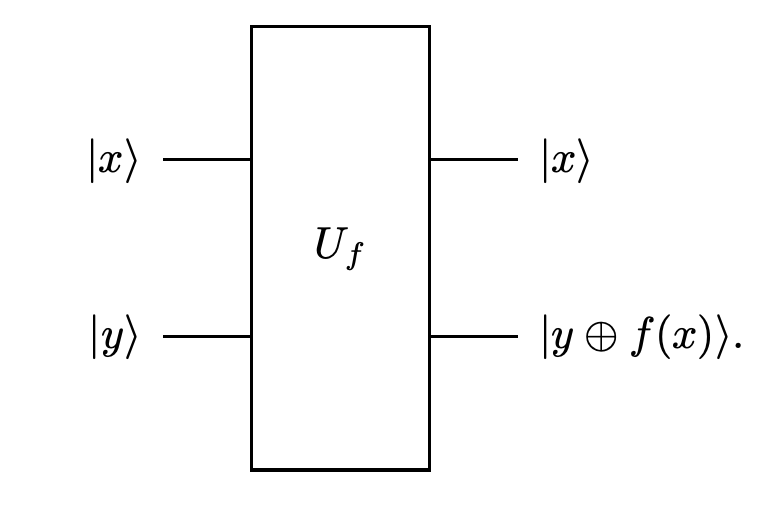
\includegraphics[width=0.5\linewidth]{pics/Gatearray.png}
    \caption{Circuit diagram of quantum gatearray.  \cite{rieffel1998introduction}}
    \label{fig:gatearray}
\end{figure}
\end{defn}
\section{EPR Paradox}
\begin{defn}[The Parity Game]
 Alice and Bob are very far apart. Each receives a random bit, say $x, y$ respectively. After seeing their random bits, each must provide a bit, say $a, b$. Alice and Bob win if
 \begin{equation}
     a \oplus b = x \land y
 \end{equation}
where $\oplus$ is XOR. To win, Alice and Bob must agree unless $x=y=1$. 
\end{defn}
 
Most of the time, Alice and Bob want to agree. In the classical setting, a good strategy is to agree always. In fact, it is optimal. Assuming they are too far apart to conspire, their disagreement is essentially random. So, if Alice and Bob disagree some of the time, then conditioning on their disagreement they will lose more often than not ($\nicefrac{3}{4}$ of the time). They could increase their expected score by reducing the chance of disagreement. 

In the quantum case, Alice and Bob can use entanglement to conspire over long distances. To demonstrate this, we will use $\ket{\to}$ for $0$ and $\ket{\uparrow}$ for $1$. Because superpositions live on the unit circle, we can picture them as rotations like $\ket{\nearrow}$.
\begin{enumerate}
    \item Construct a two qubit system in the entangled "EPR" state:
    \begin{equation}
        (\nicefrac{1}{\sqrt{2}})(\ket{\to \to} + \ket{\uparrow \uparrow})
    \end{equation}
    \item Before Alice and Bob are separated, give Alice the first EPR bit, and Bob the second EPR bit.
    \item Alice receives her random bit. If $1$, Alice applies a rotation by $\nicefrac{\pi}{8}$ to her qubit (without measuring). States are either 
    % TODO: fix formulas in this \item
    %$\ket{\rotatebox[origin=c]{22.5}{\to} \to}$ or$\ket{\ \rotatebox[origin=c]{112.5}{\to} \uparrow}$. 
    \item Bob receives his random bit and rotates by $-22.5$ if he receives a $1$.
    \item Alice and Bob read their qubits and output the bit they measure.
\end{enumerate}
Alice and Bob will now disagree some of the time, \textit{in a way that is correlated with $x\land y$}.
\begin{figure}
    \centering
    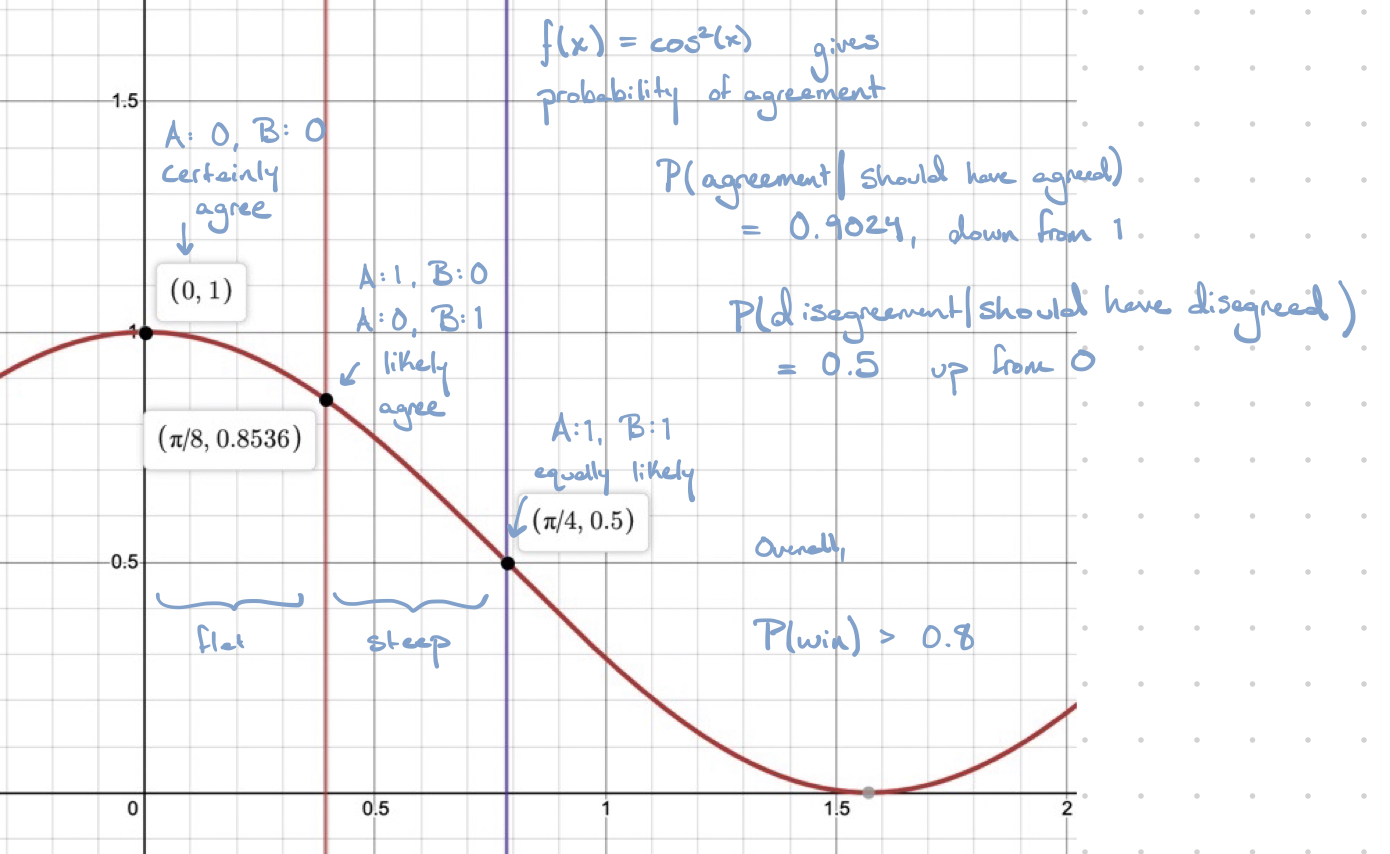
\includegraphics[width=\textwidth]{pics/EPR_Diagram.jpeg}
    \caption{EPR Diagram. $(\nicefrac{1}{4})(\nicefrac{1}{2}) > (\nicefrac{3}{4})(\nicefrac{1}{10})$, and the difference is $0.05$, which is the payoff for using this correlation strategy.}
    \label{fig:epr_diagram}
\end{figure}
\section{Dense Coding}
Using a similar idea, Alice and Bob can deterministically communicate two bits using one qubit (and one pre-shared EPR bit). 

Here is the algorithm:
\begin{enumerate}
    \item Alice and Bob each receive one bit of a prepared EPR state $\phi_0 = (\nicefrac{1}{\sqrt{2}})(\ket{00} + \ket{11})$.
    
    \item Alice receives two classical bits, encoding a number $0$ to $3$. Depending on the value, she will perform one of $\Set{I, X, Y, Z}$:
    
    \begin{tabular}{l|l|l}
         Value & Transformation & New State \\ \hline
          $0$ & $\phi_0$ = $(I \otimes I) \phi_0$ &  $(\nicefrac{1}{\sqrt{2}})(\ket{00} + \ket{11})$ \\
          $1$ & $\phi_1$ = $(I \otimes X) \phi_0$ &  $(\nicefrac{1}{\sqrt{2}})(\ket{10} + \ket{01})$ \\
          $2$ & $\phi_2$ = $(I \otimes Y) \phi_0$ &  $(\nicefrac{1}{\sqrt{2}})(-\ket{10} + \ket{01})$ \\
          $3$ & $\phi_3$ = $(I \otimes Z) \phi_0$ &  $(\nicefrac{1}{\sqrt{2}})(\ket{00} - \ket{11})$ 
    \end{tabular}
    
    \item Bob receives one of $\Set{\phi_0, \phi_1, \phi_2, \phi_3}$. He applies a $C_{not}$, \textit{which transforms all of these states to independent states}:
    
    
    \begin{tabular}{l|l|l}
         Initial State & After $C_{not}$ & Independent State \\ \hline
          $\phi_0 = (\nicefrac{1}{\sqrt{2}})(\ket{00} + \ket{11})$ & $(\nicefrac{1}{\sqrt{2}})(\ket{00} + \ket{10})$ & $(\nicefrac{1}{\sqrt{2}})(\ket{0} + \ket{1})\otimes \ket{0}$  \\
          
          $\phi_1 = (\nicefrac{1}{\sqrt{2}})(\ket{10} + \ket{01})$ & $(\nicefrac{1}{\sqrt{2}})(\ket{11} + \ket{01})$ & $(\nicefrac{1}{\sqrt{2}})(\ket{0} + \ket{1})\otimes \ket{1}$  \\
          
          $\phi_2 = (\nicefrac{1}{\sqrt{2}})(-\ket{10} + \ket{01})$ & $(\nicefrac{1}{\sqrt{2}})(-\ket{11} + \ket{01})$ & $(\nicefrac{1}{\sqrt{2}})(\ket{0} - \ket{1})\otimes \ket{1}$  \\
          
          $\phi_3 = (\nicefrac{1}{\sqrt{2}})(\ket{00} - \ket{11})$ & $(\nicefrac{1}{\sqrt{2}})(\ket{00} - \ket{10})$ & $(\nicefrac{1}{\sqrt{2}})(\ket{0} - \ket{1})\otimes \ket{0}$  
    \end{tabular}
    
    \item Bob reads the second bit (without disturbing the first bit). 
    \item By inspection, the first bit is now in an output state of the Hadamard transformation. By unitarity, $H = H^{-1}$, so Bob recovers the first bit by applying $H$ and measuring it.
\end{enumerate}
\section{BQP vs. BPP}
Classically, parallelism can be used for faster computation, but one needs exponentially many parallel processes for exponential speedup. In quantum systems, the amount of parallel computation increases exponentially with the size of the system. 

The catch is that access to the results is restricted. "we can only read the result of one parallel thread, and because measurement is probabilistic, we cannot even choose which one we get."

Quantum computation is readily analogous to \texttt{BPP}. In \texttt{BPP}, we have exponentially many computation paths, and choosing any one of them randomly is likely to give the correct answer. \textit{This is physically realizable with a quantum computer}: 
\begin{enumerate}
    \item Encode the Turing Machine $M(x) \to \Set{0, 1}$ as a quantum circuit with input $\ket{x0^{p(|x|)}}$
    \item The end padding represents the "random seed," and behavior of the circuit is deterministic based on the seed.
    \item Using linearly many Hadamard transformations, map $\ket{x0^{p(|x|)}}$ to a uniform superposition over all random seeds.
    \item Run the quantum circuit (polynomial time) and choose an output at random. By the \texttt{BPP} assumption, this output is likely to be correct.
\end{enumerate}

\begin{defn}[BQP]
A language $L$ is in \texttt{BQP} iff there exists a polynomial-time uniform family of quantum circuits $\Set{Q_n : n \in \N}$ such that
\begin{enumerate}
    \item For all $n \in \N$, $Q_n$ takes $n$ qubits as input and outputs $1$ bit
    \item For all $x \in L$, $Pr(Q_{|x|}(x) = 1) \geq \nicefrac{2}{3}$
    \item For all $x \not \in L$, $Pr(Q_{|x|}(x) = 0) \geq \nicefrac{2}{3}$
\end{enumerate}
\end{defn}

\textit{Circuit uniformity requires that the descriptions of each circuit be computable by a Turing machine of some restricted time/space. A polynomial-time uniform circuit family is computable by a polynomial time Turing machine.}


\section{Quantum Algorithms: Around Shor}

In this section we present central ideas employed by the Shor's 
algorithm for factoring integers, and a couple of designs that use those 
ideas to solve less exciting but in some sense similar problems.

We start with giving two observations that are applied
in various approaches to the problem of factorization. First, full 
factorization of a positive integer $N$ can be efficiently reduced to 
finding a factor of $N$ because there are at most $\log N$ such factors. 
Second, less trivial and the most interesting for us, finding a factor of $N$,
by the virtue of number theory, can be reduced to finding the \emph{order} of a
random number $A$, e.g., such $r < N$ that $A^r \equiv 1 \Mod N$.

There is one particular property of the mapping
\[
  b \mapsto A^b \Mod N, \qquad b\in\Z,
\]
that makes it especially interesting target for a quantum computing design. Namely,
this function is periodic (this is obvious due to finiteness of the range). The 
central task when factoring $N$ is to (efficiently) find the period $r$ of this function.

Let us step back and think what is necessary to study periodic functions in general.
First and foremost, the domain of the function should have the structure of a
group. A function $f\colon G \to X$ is periodic with period $r\in G$ ($r\neq e$) if:
\[
   \forall n\in\Z\: \forall g\in G\colon f(g+rn) = f(g).
\]

The group we are dealing with in the factoring problem is $\Z_{\phi(N)}$.
Let us consider the study of periodic functions in simpler groups:
$\Z_2$ (Deutsch problem) and $\Z^n_2$ (Simon's problem).

\subsection{Deutsch Problem}

If a function is defined on the domain $\Z_2$, there is only one possibility for period: 
$r=1$,
and the notion of periodic function here coincides with that of constant function. 
We assume that the range of functions of interest is also $\Z_2$ for convenience. 
Then all functions $f\colon \Z_2 \to \Z_2$ can be divided into two groups: constant 
functions ($f(0) \oplus f(1) = 0$) and so called  balanced functions ($f(0) \oplus f(1) = 1$).

Deutsch problem asks what it takes for a given black-box function $f$ to 
tell if it is constant or balanced?
Classically, this requires two calls to $f$. 
Deutsch algorithm solves
this problem with just one call to (a quantum realization of) $f$.

\begin{figure}
    \centering
    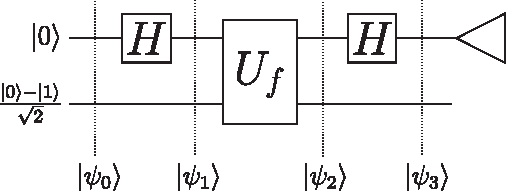
\includegraphics[width=0.8\linewidth]{pics/deutsch.pdf}
    \caption{A circuit implementing the Deutsch algorithm.}
    \label{fig:deutsch}
\end{figure}

Deutsch algorithm is provided by the circuit on Fig.~\ref{fig:deutsch}.
Here are all the intermediate states marked on the figure with normalizing 
multipliers omitted for brevity:
\begin{align*}
  \ket{\psi_0} &= \ket{0} ( \ko - \ki ),\\
  \ket{\psi_1} &= \sum_{x \in \Z_2}\ket{x} (\ko - \ki),\\
  \ket{\psi_2} &= \sum_{x \in \Z_2} (-1)^{f(x)}  \ket{x} (\ldots), \qquad \text{// qubit 2 don't matter anymore} \\ 
               &= (-1)^{f(0)}(\ko + (-1)^{f(0)\oplus f(1)}\ki)(\ldots),\\
  \ket{\psi_3} &=
    \begin{cases}
    \ko(\ldots), & \text{if $f$ is constant,}\\
    \ki(\ldots), & \text{if $f$ is balanced.}
    \end{cases}
\end{align*}
Therefore, we measure $0$ on the first wire if $f$ is constant or $1$
if it is balanced.

\subsection{Simon's Problem}

Simon's problem studies the period of a function defined on $\Z^n_2$.
In particular,
assume a black-box for computing an unknown function $f\colon \Z^n_2 \to X$ with 
the property that there exists $\bar s$, s.t.: $f(\bar x) = f(\bar y)$ iff 
$\bar x = \bar y$ or $\bar x = \bar y \oplus \bar s$.
From this, determine $\bar s$ by making queries to $f$.

\begin{figure}
    \centering
    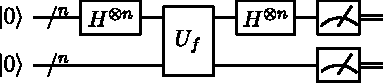
\includegraphics[width=0.8\linewidth]{pics/simon.pdf}
    \caption{A circuit implementing Simon's algorithm.}
    \label{fig:simon}
\end{figure}

There is no classical algorithm asymptotically better then brute force. This requires
exponentially many queries to $f$. A quantum solution needs only polynomially many 
steps and gates. The circuit from Fig.~\ref{fig:simon} shows the main part of the algorithm.
Here is the sequence of steps performed by the circuit:
\begin{align*}
      \ket {0^{2n}}
        \xmapsto{(1)} & \text{ // first Hadamard}\\
          \sum_{\bar x \in \Z^n_2} \ket {\bar x \,0^n}
        \xmapsto{(2)} &\text{ // $U_f$}\\\
          \sum_{\bar x \in \Z^n_2} 
            \ket {\bar x} \ket{f(\bar x)}
        \xmapsto{(3)} &\text{ // measure last $n$ qbits}\\\
          (\ket {\bar x} + \ket {\bar x \oplus \bar s}) \ket{f(\bar x)}
        \xmapsto{(4)} &\text{ // second Hadamard}\ldots
\end{align*}
To figure out how the second Hadamard acts, we use the following fact. 
\begin{exercise*}
  \[
    H^{\otimes n}(\ket{\bar x} + \ket{\bar x \oplus \bar s}  ) =
      \sum_{\bar z \in {\bar s}^\perp} (-1)^{\bar x \cdot \bar z} \ket{\bar z}.
  \]
\end{exercise*}

Therefore, the last step of the circuit will produce a random bit-string
that is orthogonal to $\bar s$. Several applications (linear in $n$)
 of the circuit will
allow us to form a non-degenerate system of linear equations that we are
able to solve on the classical computer efficiently.

\nocite{rieffel1998introduction} \nocite{arora09computationalcomplexity}
\nocite{kaye07}
\printbibliography
\end{document}
